% label prefix for this part: pm
\part{Projektmanagement}

\chapter{Vorgehensmodell}
Als Vorgehensmodell für die \acl{ba} wurde Scrum verwendet. Scrum ist ein agiles, iteratives Modell, welches sich aufgrund dessen Einfachheit und nicht besonders strikter Vorgaben sehr gut für kleinere, gut überschaubare Projekte eignet. Scrum basiert wie viele andere agile Projektmanagementmethoden auf den vier Grundsätzen die im Agilen Manifest~\cite{agilemanifesto} beschrieben sind:

\begin{itemize}
	\item Individuals and interactions over processes and tools
	\item Working software over comprehensive documentation
	\item Customer collaboration over contract negotiation
	\item Responding to change over following a plan
\end{itemize}

Wobei der Punkt \blockquote{Working software over comprehensive documentation} aufgrund der Tatsache, dass es sich um eine akademische Arbeit handelt, vernachlässigt wird.

\section{Rollen}
\mytable{lX}{
	\textbf{Rolle}  & \textbf{Beschreibung}\\
	\midrule
	
	\textbf{Product Owner} & Der Product Owner bestimmt die Anforderungen (User Stories) und priorisiert diese. Die Priorität gibt an, welche User Stories es im nächsten Sprint zu erledigt gilt.\\
	
	\textbf{Team} & Das Team besteht aus allen für das Projekt tätige Entwickler.\\
	
	\textbf{Scrum Master} & Der Scrum Master kümmert sich um die fortlaufende Kontrolle des Fortschritts sowie Optimierungsmöglichkeiten. In der Praxis ist er zudem für die Leitung der Daily Scrum Meetings, welche in diesem Projekt wegfallen, zuständig.\\
}{Scrum Projektrollen}{scrum-roles}

\section{Artefakte}
\mytable{lX}{
	\textbf{Artefakt}  & \textbf{Beschreibung}\\
	\midrule
	
	\textbf{Product Backlog} & Der Product Backlog enthält alle noch nicht abgeschlossenen User Stories des Projekts. Vor Beginn des neuen Sprints werden die noch offenen User Stories vom Product Owner repriorisiert und dessen Aufwand vom Team geschätzt.\\
	
	\textbf{Sprint Backlog} & Der Sprint Backlog enthält alle für einen bestimmten Sprint ausgewählte User Stories. Das Team setzt die Quantität fest und der Product Owner bestimmt den Inhalt und somit welche User Stories in den nächsten Sprint einfliessen.\\
	
	\textbf{Burndown Charts} & Mittels Jira werden laufend die Ist- und Sollstunden des Sprints addiert und daraus ein regressives Diagramm erstellt. Dies soll aufzeigen wie man zeitlich steht um mögliche Zeitprobleme zu vermeiden.\\
}{Scrum Artefakte}{scrum-artifacts}

\section{Sprints}

Die Iterationen, bei Scrum Sprint genannt und in \cref{fig:scrum} dargestellt, dauerten mit Ausnahme der ersten Woche jeweils zwei Wochen. So konnte, wie bei Scrum üblich, zum Ende jedes Sprints ein Deliverable, sei es eine lauffähige Applikation oder ein anderes Resultat, zur Verfügung gestellt werden.

\begin{figure}[H]
	\centering
	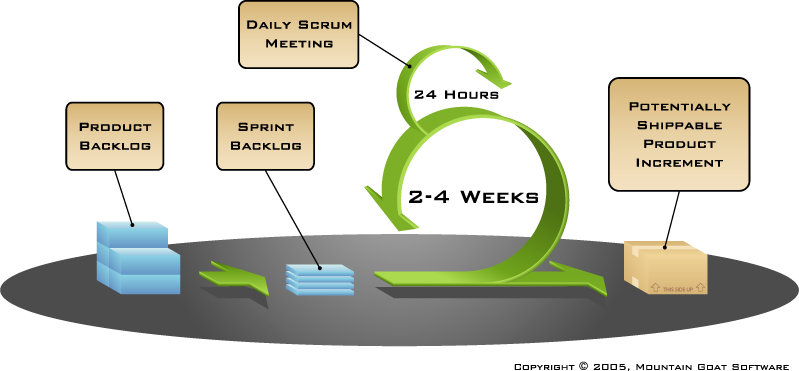
\includegraphics[width=0.7\linewidth]{fig/scrum}
	\caption[Scrum Sprint]{Scrum Sprint \cite{scrum}}
	\label{fig:scrum}
\end{figure}


\chapter{Rollen und Verantwortlichkeiten}

\section{\proff}

\begin{minipage}[t]{0.25\textwidth}
	\vspace{0pt}
	
\includegraphics[width=0.8\textwidth]{fig/sfkeller}
\end{minipage}
\begin{minipage}[t]{0.8\textwidth}
	\vspace{0pt}
	\prof, Mitarbeiter des \gls{ifs} und Dozent an der \gls{hsr} übernimmt im Projekt eine Doppelrolle:
	\begin{itemize}
		\item Als Experte bzw. Betreuer übernimmt er eine die Aufsicht und Bewertung der \acl{ba}
		\item und als fiktiver Kunde die Kontaktperson zur Aufnahme der Anforderungen (Product Owner).
	\end{itemize}
\end{minipage}


\section{\rlif}
\xxx[remo]
\begin{minipage}[t]{0.25\textwidth}
	\vspace{0pt}
	%\includegraphics[width=0.8\textwidth]{fig/rliebi}
\end{minipage}
\begin{minipage}[t]{0.8\textwidth}
	\vspace{0pt}
	\rlif, \lipsum[1]
\end{minipage}

\section{\chuf}
\xxx[christoph]
\begin{minipage}[t]{0.25\textwidth}
	\vspace{0pt}
	%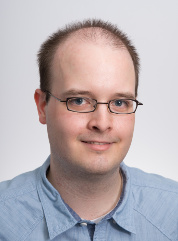
\includegraphics[width=0.8\textwidth]{fig/chuesler}
\end{minipage}
\begin{minipage}[t]{0.8\textwidth}
	\vspace{0pt}
	\chuf, \lipsum[1]
\end{minipage}


\section{\fscf}
\begin{minipage}[t]{0.25\textwidth}
	\vspace{0pt}
	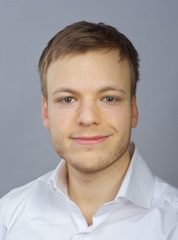
\includegraphics[width=0.8\textwidth]{fig/fscala}
\end{minipage}
\begin{minipage}[t]{0.8\textwidth}
	\vspace{0pt}
	\fscf, Teilzeitstudent an der \gls{hsr} und Banking Software Engineer bei Swisscom IT Serivces, ist Teil des Entwicklungsteams und übernimmt zusätzlich die Rolle des Scrum Masters.
\end{minipage}

\chapter{Risiken}\label{sec:risiken}

Für die Abschätzung der Projektrisiken wurde auf existierende \cite{risk} Risikochecklisten gesetzt um möglichst keine potenziellen Risiken bei der Analyse auszulassen. Die sehr umfangreiche Risikoliste von \citeauthor{Wallace:2004:SPR:975817.975819} \cite{Wallace:2004:SPR:975817.975819} wurde mit den bekannten Top Zehn Software-Projektrisiken aus dem Jahre \citeyear{boehm} \cite{boehm} sowie mit eigenen, Projektspezifischen Risiken ergänzt.
Auch die aus der Sicht des Teams, für das Projekt nicht relevante Risiken, wurden protokolliert und gelten als Nachweis, dass auch diese miteinbezogen und nicht etwa ignoriert oder gar vergessen wurden.

\begin{landscape}
	\begin{table}[H]
		\centering
		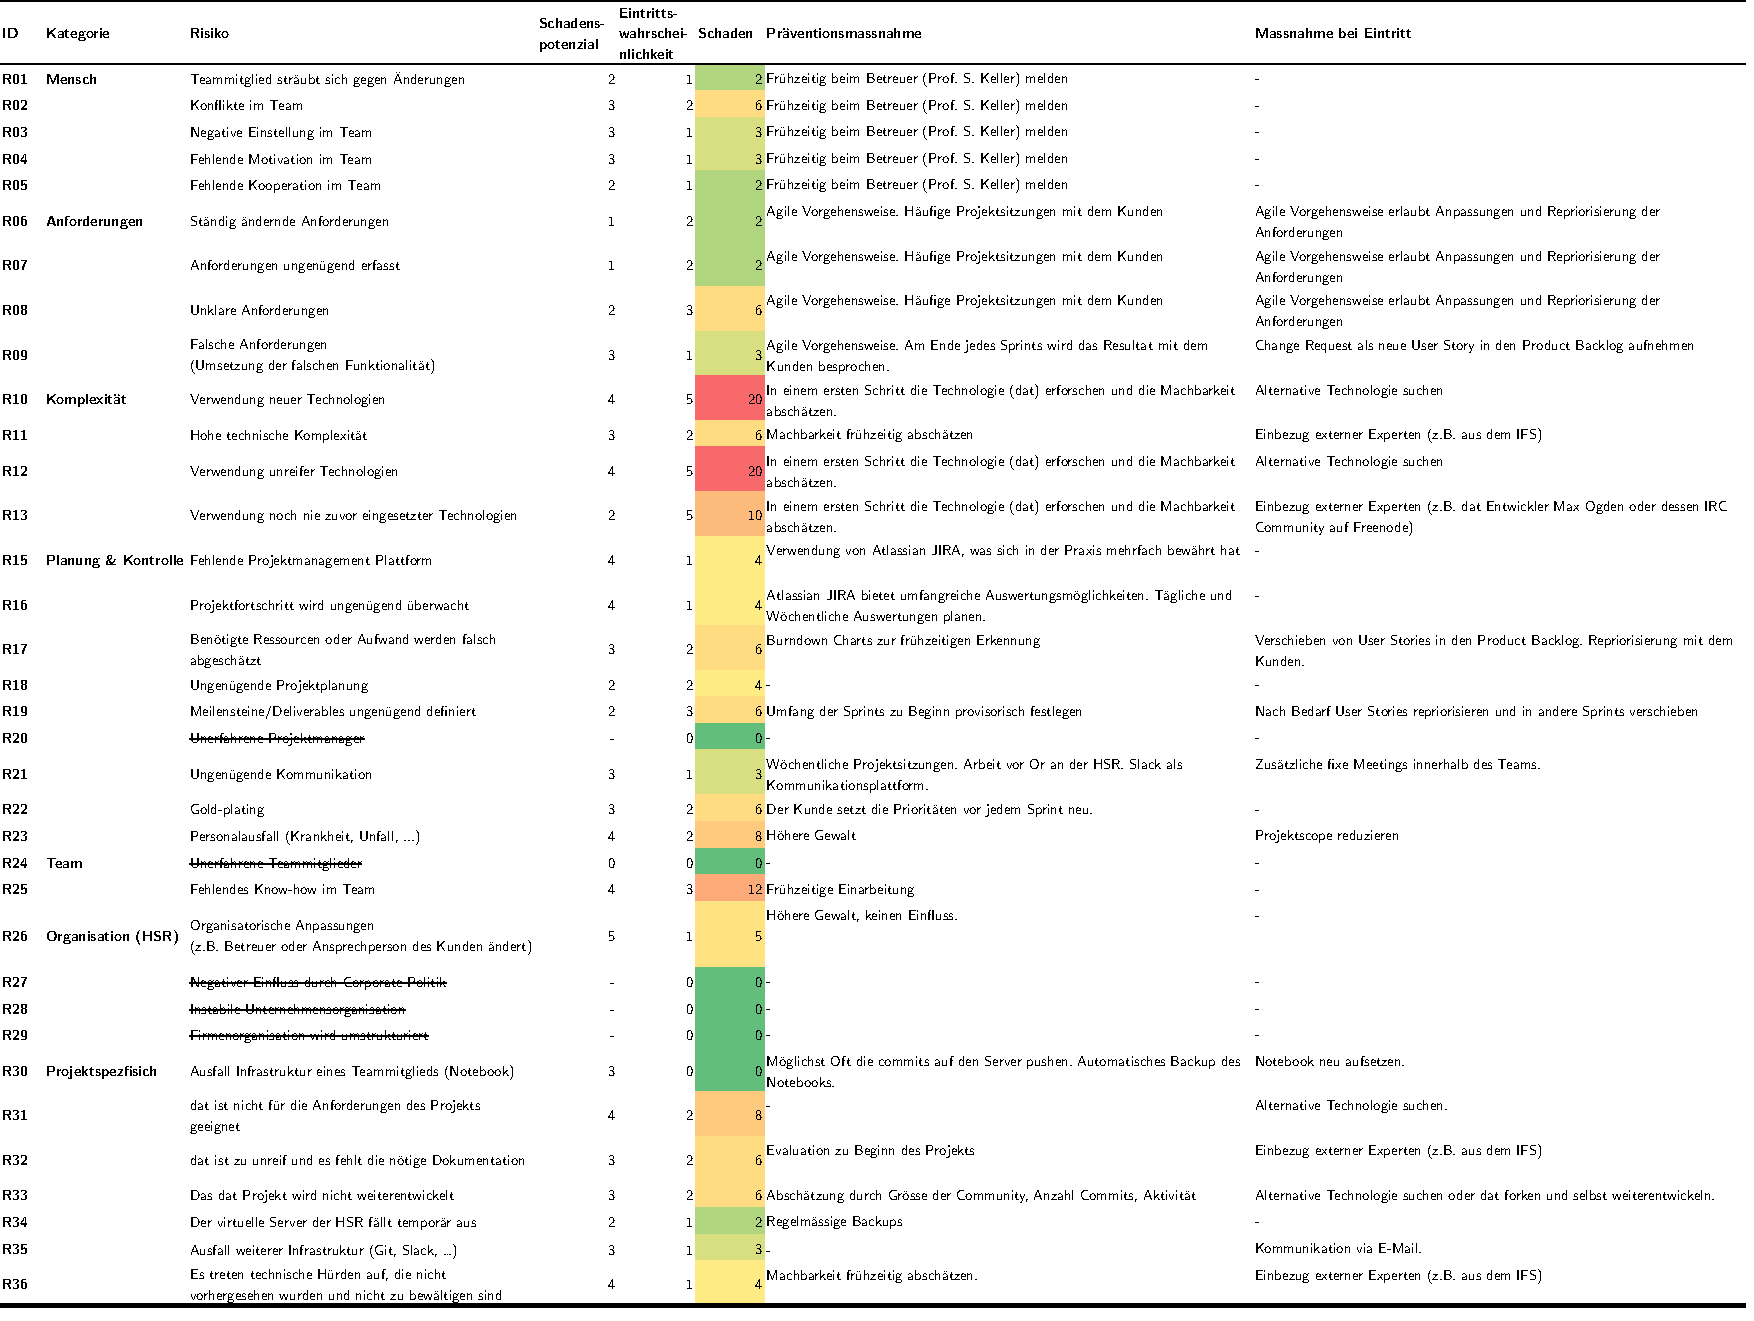
\includegraphics[height=.9\textheight,keepaspectratio]{risikoanalyse.pdf}
		\caption{Alle berücksichtigten Risiken}
		\label{tab:risikoanalyse}
	\end{table}
\end{landscape}



\section{Kritische Risiken}
Nach bzw. während der Einarbeitung in \gls{dat} wurde eine erste Abschätzung der Risiken vorgenommen. Alle irrelevanten oder ausschliessbare Risiken wurden dabei einer Eintrittswahrscheinlichkeit und Schadenspotenzial von 0 bewertet.

Nachfolgend werden die als besonders kritisch eingestuften Risiken sowie deren Massnahmen genauer beschrieben. Schon jetzt ist klar, dass das grösste Risiko das Projekt \gls{dat} selbst darstellt.


\newcommand{\projectrisk}[4]{
\begin{tabularx}{\linewidth}{lX}
	\toprule
	\textbf{Risiko} & #1\\
	\midrule
	\textbf{Titel} & #2\\
	\textbf{Beschreibung} & #3\\
	\textbf{Prävention/Massnahme} & #4\\
	\bottomrule
\end{tabularx}	
}


\projectrisk{R02}{Konflikte im Team}
{Das Projektteam kennt sich erst seit kurzem und hat davor noch nie zusammengearbeitet. Somit besteht ein erhöhten Risiko von Meinungsverschiedenheiten während des Projektverlaufs.}
{Frühzeitige Kontaktaufnahme mit dem Betreuer falls die Konflikte nicht intern gelöst werden können.}

\projectrisk{R10, R12, R13}{Verwendung neuer oder unreifer Technologien}
{Es werden unreife ``bleeding Edge'' Technologien verwendet welche die Entwicklung und Handhabung erheblich erschweren. Siehe auch \gls{dat}-spezifische Risiken R31, R32 und R33.}
{Es werden vor allem Technologien verwendet die dem Team bereits bekannt sind oder das Risiko durch eine Kurzevaluation reduziert.}

\projectrisk{R31}{\gls{dat} erfüllt nicht die Anforderungen}
{\gls{dat} und dessen Funktionalität ist nur sehr spärlich beschrieben. Selbst dem Auftraggeber ist der Umfang von \gls{dat} nicht vollständig bekannt. Es besteht das Risiko, dass \gls{dat} sich nicht für die Use Cases der Aufgabenstellung eignet.}
{Da es sich bei dieser Arbeit unter Anderem spezifisch um eine Evaluation von \gls{dat} und dessen Möglichkeiten handelt, ist eine Evaluation von alternativen Technologien zunächst zu vermeiden. Durch eine frühzeitige Einarbeitung in \gls{dat} mit kleineren Prototypen/Use Cases soll die Machbarkeit abgeschätzt werden.}


\projectrisk{R32}{\gls{dat} ist zu unreif. Fehlende Dokumentation.}
{\gls{dat} besitzt viele unbekannte Fehler und die Dokumentation ist unzureichend. Bereits während des ersten Sprints hat die spärliche Dokumentation von \gls{dat} zu Bedenken im Team geführt.}
{Dasselbe wie bei R31}


\projectrisk{R33}{\gls{dat} wird nicht weiterentwickelt}
{Der Kernentwickler von \gls{dat} (Max Ogden) verliert das Interesse am Projekt und \gls{dat} wird auch nicht von der Community nicht weiterentwickelt.}
{Abschätzung des Risikos durch die Aktivitäten der Entwickler sowie der grösse der Community. Da \gls{dat} Grundsätzlich durch die Aufgabenstellung vorgegeben ist, kann dieses Risiko nicht vermieden werden.}


\section{Risikoüberwachung}

Die Risiken wurden während des gesamten Projektverlaufs periodisch überwacht und Änderungen entsprechend protokolliert. Idealerweise sollten die Risiken über Zeit hinweg sinken.

\subsection{1. März 2015}

Wie sich herausgestellt hat, ist \gls{dat} noch weit davon entfernt um es produktiv Verwenden zu können. Ständige API Änderungen und fehlende Dokumentation machen es zu einem untragbaren Risiko. In \vref{dec:dat:fazit} wurde gegen den Einsatz von \gls{dat} Entschieden und somit die Risisken R31 bis R33 eliminiert.




\chapter{Entwicklungsumgebung und Infrastruktur}

\section{Projektmanagement}

Zur Planung der Ressourcen und Zeit sowie Zuständigkeiten der Tasks wurde das kommerzielle Tool Atlassian Jira verwendet. Jira ist kompatibel mit Agilen Vorgehensweisen, insbesondere Scrum und erlaubt mit dessen intuitivem User Interface die Planung von Sprints sowie eine Fortschrittsüberwachung mittels Burndown Charts. \cref{fig:pm:jira-agile} zeigt das sogenannte Agile Board im ``Work'' Modus während eines Sprints. Die Kopplung von Jira mit GitHub bietet mit der Verwendung von sog. Smart Commits\footnote{Beispiel: ``DAT-18 added project risks \#time 3h \#comment first draft''\newline\url{https://confluence.atlassian.com/display/FISHEYE/Using+smart+commits}} eine noch komfortablere Möglichkeit um Aufwände zu verbuchen oder Tasks zu kommentieren oder schliessen.

\begin{figure}[H]
	\centering
	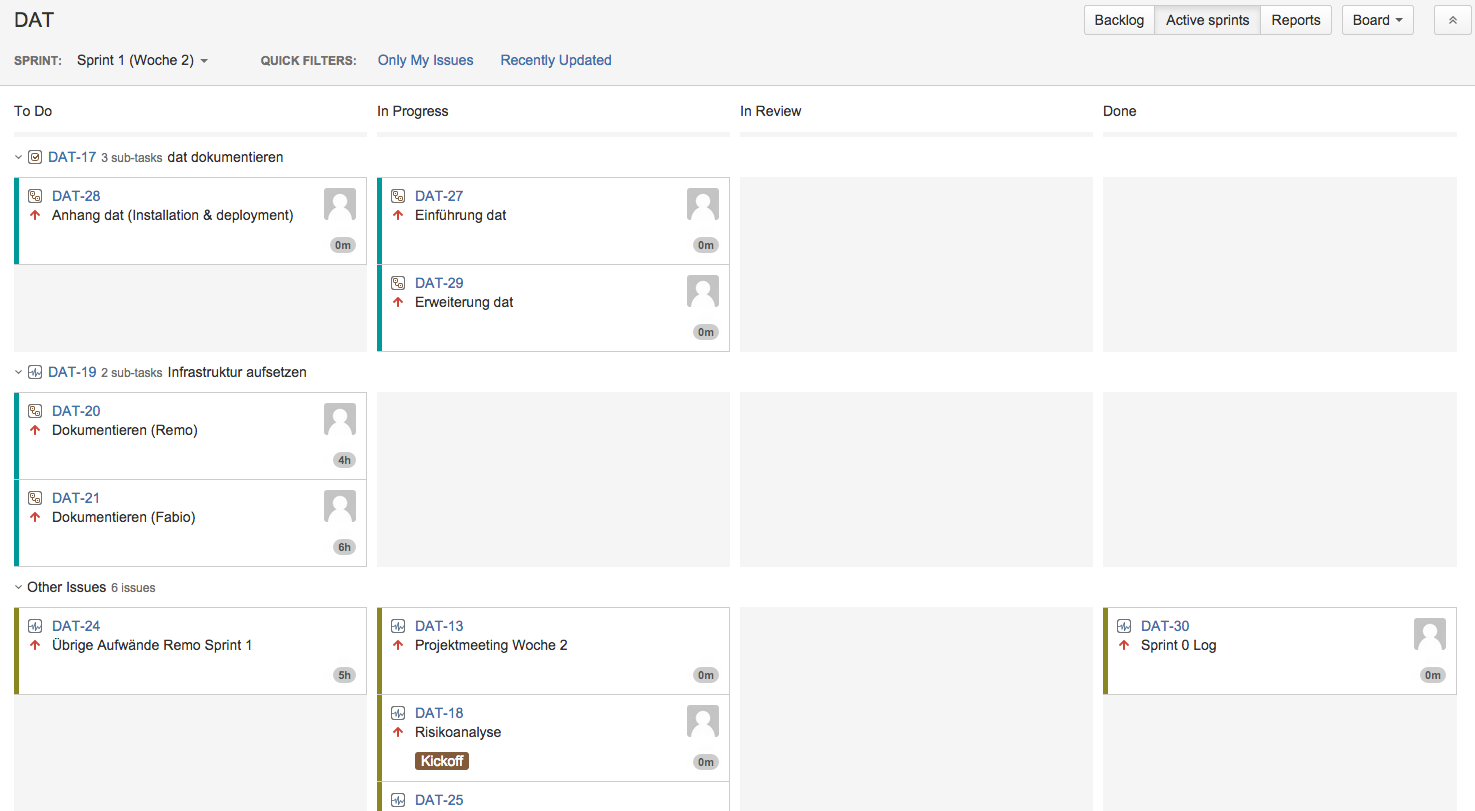
\includegraphics[width=0.95\textwidth]{fig/jira-agile}
	\caption{Jira Agile Board}
	\label{fig:pm:jira-agile}
\end{figure}

Jira wurde auf einer virtuelle Maschine der \acs{hsr} betrieben und dessen Daten täglich und automatisiert gesichert.



\section{Kommunikation}
Bei der Durchführung der Bachelorarbeit \gls{dat} wollten wir auf die Kommunikation per E-Mail verzichten. Das Team hat sich mittels \purl{http://slack.com} ausgetauscht sowie als zur Protokollierung von Sitzungen, Weblinks und weitere Informationen verwendet. Slack bietet Team-Kommunikation auf hohem Niveau, mit der Möglichkeit Services wie GitHub, Jira, Travis-CI, E-Mails usw.\footnote{\url{https://slack.com/integrations}} zu integrieren. So konnte an einem zentralen Ort Bezug auf Commits, E-Mails vom Betreuer und Failing-Builds genommen werden. Durch die Verwendung eines dedizierten Tools zur Kommunikation konnte das E-Mail Postfach von Bachelor relevanten Themen freigehalten und direkten Bezug auf konkrete Ereignisse genommen werden.

\begin{figure}[H]
	\centering
	\begin{subfigure}{0.49\textwidth}
		\centering
		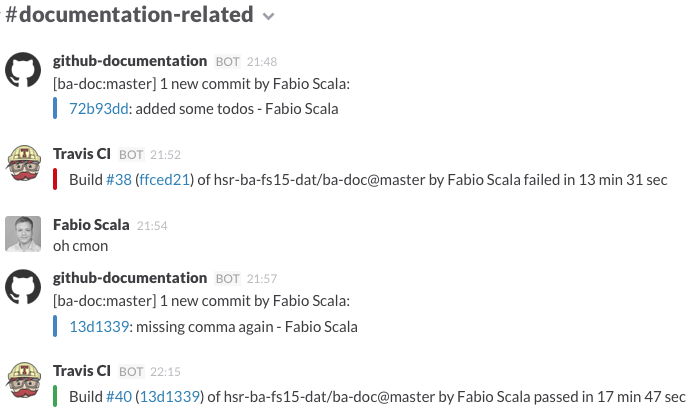
\includegraphics[width=\linewidth]{fig/slack-git-travis}
		\caption{Git und Travis}
		\label{fig:pm:slack-git-travis}
	\end{subfigure}
	\begin{subfigure}{0.49\textwidth}
		\centering
		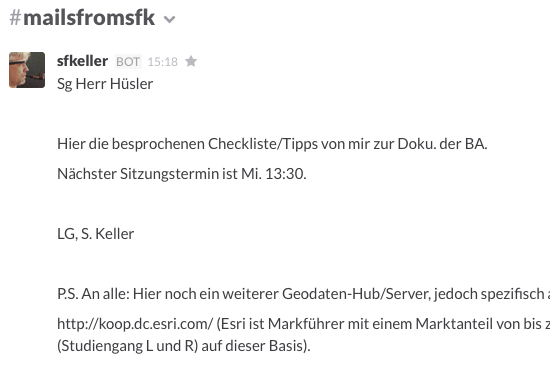
\includegraphics[width=\linewidth]{fig/slack-email}
		\caption{Automatische E-Mail Weiterleitung}
		\label{fig:pm:slack-email}
	\end{subfigure}
	\caption{Slack Screenshots}
	\label{fig:pm:slack}
\end{figure}



\chapter{Qualitätsmanagement}

\section{Reviews}

Um die Qualität der umgesetzten Tasks zu erhöhen und sicherzustellen wurde ein Review-Prozess eingesetzt. Jeder Task darf erst abgeschlossen werden, wenn ein anderes Teammitglied das Resultat grob angeschaut und für gut befunden hat. Um diesen Prozess einzuhalten wurde ein eigener Jira-Workflow verwendet.

\begin{figure}
\centering
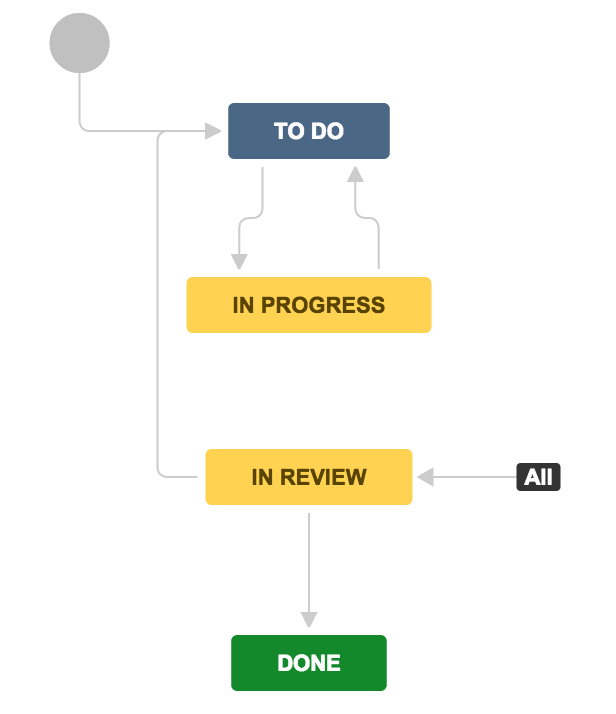
\includegraphics[width=0.7\linewidth]{fig/jira-workflow}
\caption{Jira Review-Workflow}
\label{fig:jira-workflow}
\end{figure}

Der in \cref{fig:jira-workflow} dargestellte Prozess stellt sicher, dass alle Tasks erst in den Review Status versetzt werden müssen. Von diesem Status aus kann der Task entweder durch den Reviewer geschlossen oder zurück in den Status ``To Do'' versetzt werden, wobei bei letzterem der Tasks automatisch dem ursprünglichen Teammitglied zugewiesen wird.

\pagebreak
\section{Vagrant}
\subsection{Überblick}
Vagrant ist eine auf Ruby basierte, freie Anwendung, die das Verwalten und Erstellen von virtuellen Maschinen ermöglicht. Vagrant dient eigentlich als Wrapper zwischen der Virtualisierungssoftware (Virtualbox, VMware, Parallels, etc.) und Systemkonfiguartionswerkzeugen (in unserem Fall Puppet).
Der grosse Mehrwert von Vagrant ergibt sich dadurch, dass es komplett programmiersprachenunabhängig ist und somit für verschiedene Softwareprojekte verwendet werden kann. Im Vagrantfile wird eine virtuelle Maschine definiert und konfiguriert. Dieses File wird mit dem Projekt in der Versonskontrolle abgelet, so kann auf den unterschiedlichen Host Systemen gewährleistet werden, dass mit der selben Entwicklungsumgebung gearbeitet werden kann und so alle Abhängigkeiten, ohne das Hostsystem zu beeinflussen, gewährleistet werden.
\subsection{Projektinitalisierung}
Ein Projekt wird mit folgendem Befehl initialisiert
\begin{src}{shell}
vagrant init [box-name] [box-url]
\end{src}
 Durch die Angabe des ``box-name'' kann direkt eine entsprechende Vorlage ins Vagrantfile geladen werden. Die URL kann dazu verwendet werden, den Ort an dem sich das Image befindet anzugeben, und diese direkt herunterzuladen. Diese Angaben haben wir im Vagrantfile, bzw. mittels Puppet konfiguriert.
\subsection{Konfiguration}
Die gesamte Konfiguration erfolgt im Vagrantfile. 
\begin{srclst}{ruby}{Syntax-Beispiel eines Vagrantfile (generiert von puphpet.com)}
require 'yaml'

dir = File.dirname(File.expand_path(__FILE__))

configValues = YAML.load_file("#{dir}/puphpet/config.yaml")
data         = configValues['vagrantfile-local']

Vagrant.require_version '>= 1.6.0'

Vagrant.configure('2') do |config|
  config.vm.box     = "#{data['vm']['box']}"
  config.vm.box_url = "#{data['vm']['box_url']}"

  if data['vm']['hostname'].to_s.strip.length != 0
    config.vm.hostname = "#{data['vm']['hostname']}"
  end
  [...]
end
\end{srclst}
\subsection{Provisioning}
In der Phase Provisioning werden andere Programme, zumeist SCM-Software wie aptitude, aber auch grundlegende Anwendungen wie Shell konfiguriert und parameter übergeben.
Hier ein Auszug eines unsere provisioning files:
\begin{src}{shell}
#!/bin/sh

sudo apt-get update
sudo apt-get upgrade
source ~/.bashrc
sudo wget -qO- https://toolbelt.heroku.com/install-ubuntu.sh | sh
# ------ Frontend
cd /vagrant/webapp/frontend

# Required for SASS
sudo `which gem` install compass

# Cleanup
rm -rf bower_components node_modules

# Install deps

npm install
bower install --config.analytics=false --allow-root


# ------ Backend
cd /vagrant/webapp/backend

# Cleanup
rm -rf env target

# Create virtualenv with existing packages (see config.yaml)
virtualenv --system-site-packages env
source env/bin/activate

# Install all requirements.txt and requirements_dev.txt dependencies
pyb install_dependencies

\end{src}
\subsection{Arbeiten mit Vagrant}
Um eine \gls{vm} zu starten, führt man den Befehl \mintinline{shell}{vagrant up} aus. Beim Ausführen des Befehles wird die \gls{vm} gemäss den Vorgaben im Vagrantfile initialisiert. Später kann man mittels \mintinline{shell}{vagrant ssh} per SSH direkt in die \gls{vm} verbunden werden. Wird die Maschine (vorübergehend) nicht mehr gebraucht, kann mittels \mintinline{shell}{vagrant suspend} die \gls{vm} in den Ruhezustand gebracht werden.
\subsection{Deployment}
Seit der Vagrant Version 1.7 vom Dezember 2014 ist Deployment mittels Vagrant möglich. Durch den Befehl \mintinline{shell}{vagrant push} kann, je nach Konfiguration, auf Heroku, SFTP und FTP sowie durch selbstgeschriebene Kommandozeilenskripte oder Atlas deployed werden.
\\Syntaxbeispiel für einen FTP-push: \cite{vagrant-deployment}
\begin{src}{ruby}
config.push.define "ftp" do |push|
  push.host = "ftp.test.com"
  push.username = "benutzer1"
  push.password = "Passwort1"
  push.secure = false
  push.destination = "/"
  push.dir = "/"
end
\end{src}
\section{Tests}

\section{Coding-Richtlinien}

\subsection{Python}
\xxx[pep8?]


\subsection{JavaScript}


\subsection{AngularJS}
\xxx[scaffolding, controller as, kein dom in controllern]




\subimport{sprints/}{sprints.tex}


